\documentclass[10pt,landscape,twocolumn,letterpaper]{article}

\usepackage[margin=1.27cm]{geometry}
\setlength{\textwidth}{10.0in}		% default=9in

\setlength{\columnsep}{0.5in}		% default=10pt
\setlength{\columnseprule}{0pt}		% default=0pt (no line)
%\setlength{\columnseprule}{0.2pt}		% default=0pt (no line)

\setlength{\textheight}{7in}		% default=5.15in
\setlength{\topmargin}{-.5in}		% default=0.20in

\setlength{\headsep}{0in}		% default=0.35in

\setlength{\parskip}{1.2ex}
\setlength{\parindent}{0mm}
\usepackage{graphicx}
\usepackage{paralist} 
%\usepackage{helvetica,color}
%\usepackage{newcent,color}
%\usepackage{bookman,color}
\usepackage{palatino}
\usepackage{color}
\usepackage{stmaryrd}
\pagestyle{empty}

\begin{document}
%\maketitle

\begin{center}
\textbf{Deuteronomy}
\end{center}
DEUTERONOMY consists of the parting counsels of Moses delivered to Israel upon the impending entrance upon their covenanted possession. It is important to note that, while the land of promise was unconditionally given Abraham and to his seed in the Abrahamic Covenant (Genesis 13:15 ; 15:7), it was under the conditional Palestinian Covenant (Deuteronomy 28:1-30:9) that Israel entered the land under Joshua. Utterly violating the conditions of that covenant, the nation was first disrupted (1 Kings 12) and then cast out of the land (2 Kings 17:1-18 ; 24:1-25:11). But the same covenant unconditionally promises a national restoration of Israel which is yet to be fulfilled (See Scofield).  The time covered by this retrospect is approximately forty years.
 
\begin{tabular}{p{0.7in}p{0.7in}p{1.8in}p{0.55in}}
  %\hline
  % after \\: \hline or \cline{col1-col2} \cline{col3-col4} ...
  DAY & CH & COMMENTS &  \\

\tiny 060 \normalsize \textcolor[rgb]{0.00,0.00,1.00}{Tue, $1^{st}$} & \textcolor[rgb]{0.00,0.00,1.00}{Deut 25-27} & \textcolor[rgb]{0.50,0.50,0.50}{\small Conquering Transjordan} & $\boxempty$ $\boxempty$ $\boxempty$\\


\tiny 061 \normalsize \textcolor[rgb]{0.00,0.00,1.00}{Wed, $2^{nd}$} & \textcolor[rgb]{0.00,0.00,1.00}{Deut 28-30} & \textcolor[rgb]{0.50,0.50,0.50}{\small Cities of Refuge} & $\boxempty$ $\boxempty$ $\boxempty$\\
     & \multicolumn{2}{l}{\textcolor[rgb]{1.00,0.00,0.00}{Psalm 26 -- The Crucifixion Psalm}} & $\boxempty$ \\

\tiny 062 \normalsize \textcolor[rgb]{0.00,0.00,1.00}{Thu, $3^{rd}$} & \textcolor[rgb]{0.00,0.00,1.00}{Deut 31-34} & \textcolor[rgb]{0.50,0.50,0.50}{\small Remembering the Lord's Doings} & $\boxempty $ $\boxempty$ $\boxempty$ $\boxempty$\\

\end{tabular}

\begin{center}
\textbf{Joshua}
\end{center}
JOSHUA records the consummation of the redemption of Israel of Israel out of Egypt; for redemption has two parts: ``out,'' and ``into'' (Deuteronomy 6:23). In a spiritual sense the book of Joshua is the Ephesians of the Old Testament. ``The heavenly'' of Ephesians is to the Christian what Canaan was to the Israelite and blessing through divine power (Joshua 21:43-55, Ephesians 1:3). 
 
\begin{tabular}{p{0.75in}p{0.65in}p{1.8in}p{0.55in}}
  %\hline
  % after \\: \hline or \cline{col1-col2} \cline{col3-col4} ...
  DAY & CH & COMMENTS &  \\
\tiny 063 \normalsize \textcolor[rgb]{0.00,0.00,1.00}{Fri, $4^{th}$} & \textcolor[rgb]{0.00,0.00,1.00}{Josh 1--3} & \textcolor[rgb]{0.50,0.50,0.50}{\small Commission  \& Crossing} & $\boxempty$ $\boxempty$ $\boxempty$\\
     & \multicolumn{2}{l}{\textcolor[rgb]{1.00,0.00,0.00}{Psalm 27 -- Anthem of Praise}} & $\boxempty$ \\

\tiny 064 \normalsize \textcolor[rgb]{0.00,0.00,1.00}{Sat, $5^{th}$} & \textcolor[rgb]{0.00,0.00,1.00}{Josh 4--6} & \textcolor[rgb]{0.50,0.50,0.50}{\small Meet the Captain!} & $\boxempty$ $\boxempty$ $\boxempty$\\

\tiny 065 \normalsize \textcolor[rgb]{0.00,0.00,1.00}{Sun, $6^{th}$} & \textcolor[rgb]{0.00,0.00,1.00}{Josh 7--9} & \textcolor[rgb]{0.50,0.50,0.50}{\small Ai \& The Gibeonites} &  $\boxempty$ $\boxempty$ $\boxempty$\\

\tiny 066 \normalsize \textcolor[rgb]{0.00,0.00,1.00}{Mon, $7^{th}$} & \textcolor[rgb]{0.00,0.00,1.00}{Josh 10--12} & \textcolor[rgb]{0.50,0.50,0.50}{\small Conquest} & $\boxempty$ $\boxempty$ $\boxempty$\\
     & \multicolumn{2}{l}{\textcolor[rgb]{1.00,0.00,0.00}{Psalm 28 -- A Lament}} & $\boxempty$ \\

\tiny 067 \normalsize \textcolor[rgb]{0.00,0.00,1.00}{Tue, $8^{th}$} & \textcolor[rgb]{0.00,0.00,1.00}{Josh 13--15} & \textcolor[rgb]{0.50,0.50,0.50}{\small Dividing Canaan} & $\boxempty$ $\boxempty$ $\boxempty$\\

\tiny 068 \normalsize \textcolor[rgb]{0.00,0.00,1.00}{Wed, $9^{th}$} & \textcolor[rgb]{0.00,0.00,1.00}{Josh 16--18} & \textcolor[rgb]{0.50,0.50,0.50}{\small Dividing Canaan} &  $\boxempty$ $\boxempty$ $\boxempty$\\
     & \multicolumn{2}{l}{\textcolor[rgb]{1.00,0.00,0.00}{Psalm 29 -- A Hymn to the Omnipotent God}} & $\boxempty$ \\

\tiny 069 \normalsize  \textcolor[rgb]{0.00,0.00,1.00}{Thu, $10^{th}$} & \textcolor[rgb]{0.00,0.00,1.00}{Josh 19--21} & \textcolor[rgb]{0.50,0.50,0.50}{\small Cities of Refuge} & $\boxempty$ $\boxempty$ $\boxempty$\\

\tiny 070 \normalsize  \textcolor[rgb]{0.00,0.00,1.00}{Fri, $11^{th}$} & \textcolor[rgb]{0.00,0.00,1.00}{Josh 22--24} & \textcolor[rgb]{0.50,0.50,0.50}{\small Goodbye to Joshua} &  $\boxempty$ $\boxempty$ $\boxempty$\\
     & \multicolumn{2}{l}{\textcolor[rgb]{1.00,0.00,0.00}{Psalm 30 -- A ThanksgivingPsalm}} & $\boxempty$ \\
\end{tabular}

\newpage
\begin{center}
\textbf{Judges}
\end{center}
Judges takes its name from the thirteen men raised up to deliver Israel in the declension and disunion which followed the death of Joshua. Through these men Jehovah continued His personal government of Israel. The key-verse to the condition of Israel is (Judges 17:6), ``Every man did that which was right in his own eyes.'' Two facts stand out--the utter failure of Israel, and the persistent grace of Jehovah. In the choice of the Judges is illustrated Zechariah's great word (Zechariah 4:6), ``not by might, nor by power, but by My Spirit, saith the Lord''; and Paul's word (1 Corinthians 1:25), ``not many wise men after the flesh, not many mighty, not many noble, are called.'' The book records seven apostasies, seven servitudes to seven heathen nations, seven deliverances. The spiritual parallel is found in the history of the professing church since the Apostles, in the rise of sects and the lost sense of the unity of the one body.
\begin{tabular}{p{0.75in}p{0.7in}p{1.8in}p{0.50in}}
  DAY & CH & COMMENTS &  \\
\tiny 071 \normalsize   \textcolor[rgb]{0.00,0.00,1.00}{Sat, $12^{th}$} & \textcolor[rgb]{0.00,0.00,1.00}{Jdgs 1--3} & \textcolor[rgb]{0.50,0.50,0.50}{\small Othiel, Ehud, Samgar} & $\boxempty$ $\boxempty$ $\boxempty$\\

\tiny 072 \normalsize  \textcolor[rgb]{0.00,0.00,1.00}{Sun, $13^{th}$} & \textcolor[rgb]{0.00,0.00,1.00}{Jdgs 4--6} & \textcolor[rgb]{0.50,0.50,0.50}{\small Deborah, Barak, Gideon} & $\boxempty$ $\boxempty$ $\boxempty$\\

\tiny 073 \normalsize \textcolor[rgb]{0.00,0.00,1.00}{Mon, $14^{th}$} & \textcolor[rgb]{0.00,0.00,1.00}{Jdgs 7--9} & \textcolor[rgb]{0.50,0.50,0.50}{\small Gideon \& Abimelech} &  $\boxempty$ $\boxempty$ $\boxempty$\\
     & \multicolumn{2}{l}{\textcolor[rgb]{1.00,0.00,0.00}{Psalm 31 -- A Lament}} & $\boxempty$ \\
    
\tiny 074 \normalsize  \textcolor[rgb]{0.00,0.00,1.00}{Tue, $15^{th}$} & \textcolor[rgb]{0.00,0.00,1.00}{Jdgs 10--12} & \textcolor[rgb]{0.50,0.50,0.50}{\small Tola ... Abdon} & $\boxempty$ $\boxempty$ $\boxempty$\\


\tiny 075 \normalsize \textcolor[rgb]{0.00,0.00,1.00}{Wed, $16^{th}$} & \textcolor[rgb]{0.00,0.00,1.00}{Jdgs 13--15} & \textcolor[rgb]{0.50,0.50,0.50}{\small Samson} & $\boxempty$ $\boxempty$ $\boxempty$\\
       & \multicolumn{2}{l}{\textcolor[rgb]{1.00,0.00,0.00}{Psalm 32 -- Psalm of Forgiveness}} & $\boxempty$ \\
       
\tiny 076 \normalsize \textcolor[rgb]{0.00,0.00,1.00}{Thu, $17^{th}$} & \textcolor[rgb]{0.00,0.00,1.00}{Jdgs 16--18} & \textcolor[rgb]{0.50,0.50,0.50}{\small Danites} &  $\boxempty$ $\boxempty$ $\boxempty$\\


\tiny 077 \normalsize \textcolor[rgb]{0.00,0.00,1.00}{Fri, $18^{th}$} & \textcolor[rgb]{0.00,0.00,1.00}{Jdgs 19--21} & \textcolor[rgb]{0.50,0.50,0.50}{\small Benjamite War} & $\boxempty$ $\boxempty$ $\boxempty$\\
       & \multicolumn{2}{l}{\textcolor[rgb]{1.00,0.00,0.00}{Psalm 33 -- Hymn of Praise}} & $\boxempty$ \\
\end{tabular} 
\begin{center}
\textbf{Ruth}
\end{center}
Ruth should be read in connection with the first half of Judges, as it presents a picture of life in Israel at that time.  
Typically, the book may be taken as a foreview of the church (Ruth), as the Gentile bride of Christ, the Bethlehemite who is able to redeem. Ruth also gives a normal Christian experience: (1) Ruth deciding: 1, (2) Ruth serving: 2, (3) Ruth resting: 3, (4) Ruth rewarded: 4. The events recorded in Ruth cover a period of 10 years (Ussher)
\begin{tabular}{p{0.7in}p{0.7in}p{1.8in}p{0.55in}}
  DAY & CH & COMMENTS &  \\
\tiny 078 \normalsize  \textcolor[rgb]{0.00,0.00,1.00}{Sat, $19^{th}$} & \textcolor[rgb]{0.00,0.00,1.00}{Ruth 1--4} & \textcolor[rgb]{0.50,0.50,0.50}{\small Romance of Redemption} & $\boxempty$ $\boxempty$ $\boxempty$ $\boxempty$\\
\end{tabular}
\begin{center}
\textbf{1 \& 2 Samuel}
\end{center}
1 SAMUEL represents the personal history of Samuel, last of the Judges. It records the moral failure of the priesthood under Eli, and of the Judges in Samuel's attempt to make the office hereditary (1 Samuel 8:1). In his prophetic office Samuel was faithful, and in him begins the line of writing prophets. Henceforth the prophet, not the priest, is conspicuous in Israel. In this book the theocracy, as exercised through judges, ends (1 Samuel 8:7), and the line of kings begins with Saul. As First Samuel marks the failure of man in Eli, Saul, and even Samuel, so 2 SAMUEL marks the restoration of order through the enthroning of God's king, David. This book also records the establishment of Israel's political centre in Jerusalem (2 Samuel 5:6-12), and her religious centre in Zion (2 Samuel 5:7, 6:1-17). When all was thus ordered, Jehovah established the great Davidic Covenant (2 Samuel 27:8-17) out of which all kingdom truth is henceforth developed. David, in his ``last words'' (2 Samuel 23:1-7), describes the millennial kingdom yet to be.
\begin{tabular}{p{0.75in}p{0.8in}p{1.7in}p{0.50in}}
  %\hline
  % after \\: \hline or \cline{col1-col2} \cline{col3-col4} ...
  DAY & CH & COMMENTS &  \\
\tiny 079 \normalsize  \textcolor[rgb]{0.00,0.00,1.00}{Sun, $20^{th}$} & \textcolor[rgb]{0.00,0.00,1.00}{1Sam 1--3} & \textcolor[rgb]{0.50,0.50,0.50}{\small Samuel's Childhoodg} & $\boxempty$ $\boxempty$ $\boxempty$\\

\tiny 080 \normalsize  \textcolor[rgb]{0.00,0.00,1.00}{Mon, $21^{st}$} & \textcolor[rgb]{0.00,0.00,1.00}{1Sam 4--6} & \textcolor[rgb]{0.50,0.50,0.50}{\small War with Philistines} & $\boxempty$ $\boxempty$ $\boxempty$\\
     & \multicolumn{2}{l}{\textcolor[rgb]{1.00,0.00,0.00}{Psalm 34 -- Psalm of Thanksgiving}} & $\boxempty$ \\
     
\tiny 081 \normalsize  \textcolor[rgb]{0.00,0.00,1.00}{Tue, $22^{nd}$} & \textcolor[rgb]{0.00,0.00,1.00}{1Sam 7--9} & \textcolor[rgb]{0.50,0.50,0.50}{\small Rise of Saul} &  $\boxempty$ $\boxempty$ $\boxempty$\\

\tiny 082 \normalsize \textcolor[rgb]{0.00,0.00,1.00}{Wed, $23^{rd}$} & \textcolor[rgb]{0.00,0.00,1.00}{1Sm 10--12} & \textcolor[rgb]{0.50,0.50,0.50}{\small Saul's Adventures} & $\boxempty$ $\boxempty$ $\boxempty$\\
     & \multicolumn{2}{l}{\textcolor[rgb]{1.00,0.00,0.00}{Psalm 35 -- Imprecatory Psalm}} & $\boxempty$ \\

\tiny 083 \normalsize \textcolor[rgb]{0.00,0.00,1.00}{Thu, $24^{th}$} & \textcolor[rgb]{0.00,0.00,1.00}{1Sam 13--15} & \textcolor[rgb]{0.50,0.50,0.50}{\small Saul's Apostacy} & $\boxempty$ $\boxempty$ $\boxempty$\\

\tiny 084 \normalsize \textcolor[rgb]{0.00,0.00,1.00}{Fri, $25^{th}$} & \textcolor[rgb]{0.00,0.00,1.00}{1Sam 16--18} & \textcolor[rgb]{0.50,0.50,0.50}{\small Rise of David} &  $\boxempty$ $\boxempty$ $\boxempty$\\
     & \multicolumn{2}{l}{\textcolor[rgb]{1.00,0.00,0.00}{Psalm 36 -- A Psalm of Praise}} & $\boxempty$ \\

\tiny 085 \normalsize \textcolor[rgb]{0.00,0.00,1.00}{Sat, $26^{th}$} & \textcolor[rgb]{0.00,0.00,1.00}{1Sam 19--21} & \textcolor[rgb]{0.50,0.50,0.50}{\small Protection of David} & $\boxempty$ $\boxempty$ $\boxempty$\\

\tiny 086 \normalsize \textcolor[rgb]{0.00,0.00,1.00}{Sun, $27^{th}$} & \textcolor[rgb]{0.00,0.00,1.00}{1Sam 22--24} & \textcolor[rgb]{0.50,0.50,0.50}{\small David \& his Men} &  $\boxempty$ $\boxempty$ $\boxempty$\\

\tiny 087 \normalsize \textcolor[rgb]{0.00,0.00,1.00}{Mon, $28^{th}$} & \textcolor[rgb]{0.00,0.00,1.00}{1Sam 25--27} & \textcolor[rgb]{0.50,0.50,0.50}{\small Abigail, Wilderness} &  $\boxempty$ $\boxempty$ $\boxempty$\\
     & \multicolumn{2}{l}{\textcolor[rgb]{1.00,0.00,0.00}{Psalm 37 -- A Wisdom Psalm}} & $\boxempty$ \\

\tiny 088\normalsize \textcolor[rgb]{0.00,0.00,1.00}{Tue, $29^{th}$} & \textcolor[rgb]{0.00,0.00,1.00}{1Sam 28--31} & \textcolor[rgb]{0.50,0.50,0.50}{\small Saul's End} & $\boxempty$ $\boxempty$ $\boxempty$ $\boxempty$\\

\tiny 089 \normalsize \textcolor[rgb]{0.00,0.00,1.00}{Wed, $30^{th}$} & \textcolor[rgb]{0.00,0.00,1.00}{2Sam 1--3} & \textcolor[rgb]{0.50,0.50,0.50}{\small David's Coronation} &  $\boxempty$ $\boxempty$ $\boxempty$\\
     & \multicolumn{2}{l}{\textcolor[rgb]{1.00,0.00,0.00}{Psalm 38 -- A Penitential Psalm}} & $\boxempty$ \\

\tiny 090 \normalsize \textcolor[rgb]{0.00,0.00,1.00}{Thu, $31^{st}$} & \textcolor[rgb]{0.00,0.00,1.00}{2Sam 4--6} & \textcolor[rgb]{0.50,0.50,0.50}{\small The Ark Returns} &  $\boxempty$ $\boxempty$ $\boxempty$\\

\end{tabular}





\newpage
\LARGE
\begin{center}
\textcolor[rgb]{0.98,0.00,0.00}{Daily Bible Reading}\\
\textcolor[rgb]{0.00,0.00,1.00}{March 2021}\\
\end{center}


\begin{figure}[htp]
    \centering
  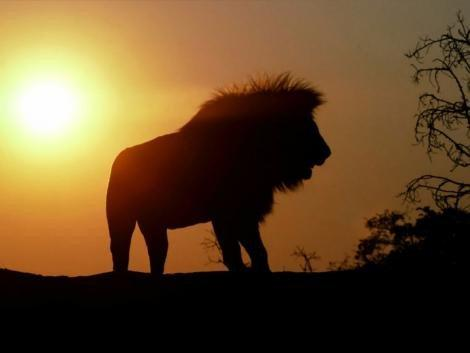
\includegraphics[width=4.5in]{March}\\
%  \caption{}\label{}
\end{figure}

\begin{center}
\textcolor[rgb]{0.00,0.00,1.00}{\\Ask Yourself ...}
\textcolor[rgb]{1.00,0.00,0.00}{\\Who is Speaking?\\Who is being spoken to?\\What is being said?\\Are there
any commandments to obey?\\Are there any promises to claim?}
\end{center}

%\vspace{0.5in}
\hfill \tiny{\textcolor[rgb]{0.50,0.50,0.50}{01/1/19}}

\end{document}
